% Made up for the tikra benchmark.
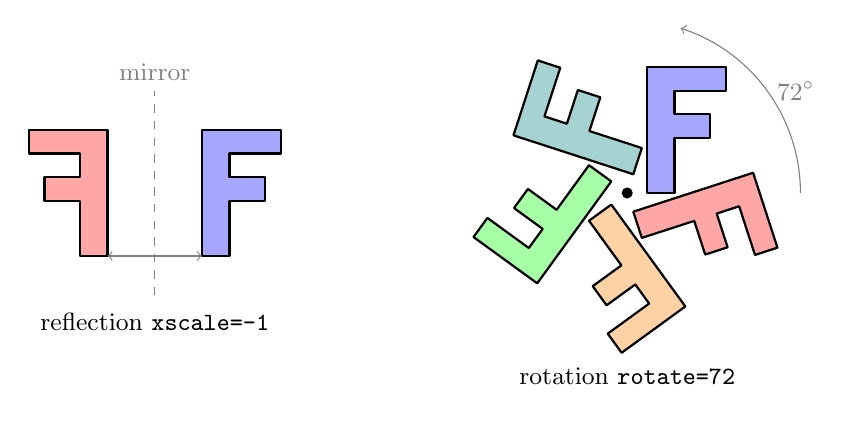
\begin{tikzpicture}[line join=round,
    flag/.pic={\draw[thick, fill=#1] (0,0) -- (0,1.6) -- (1,1.6) -- (1,1.3) -- (0.35,1.3)
                -- (0.35,1) -- (0.8,1) -- (0.8,0.7) -- (0.35,0.7) -- (0.35,0) -- cycle;}]
  % reflection across a vertical mirror
  \begin{scope}
    \draw[dashed, gray] (0,-0.4) -- (0,2.2) node[above, font=\small] {mirror};
    \pic at (0.6,0.1) {flag=blue!35};
    \begin{scope}[xscale=-1]
      \pic[transform shape] at (0.6,0.1) {flag=red!35};
    \end{scope}
    \draw[gray, <->] (0.6,0.1) -- (-0.6,0.1);
    \node[below, font=\small] at (0,-0.5) {reflection \texttt{xscale=-1}};
  \end{scope}
  % rotations about a point
  \begin{scope}[xshift=6cm, yshift=0.9cm]
    \foreach \a/\c in {0/blue!35, 72/teal!35, 144/green!35, 216/orange!35, 288/red!35} {
      \begin{scope}[rotate=\a]
        \pic[transform shape] at (0.25,0) {flag=\c};
      \end{scope}
    }
    \fill (0,0) circle (2pt);
    \draw[->, gray] (2.2,0) arc (0:72:2.2) node[midway, right, font=\small] {$72^\circ$};
    \node[below, font=\small] at (0,-2.1) {rotation \texttt{rotate=72}};
  \end{scope}
\end{tikzpicture}
